%%
%% This is file `sample-sigconf.tex',
%% generated with the docstrip utility.
%%
%% The original source files were:
%%
%% samples.dtx  (with options: `all,proceedings,bibtex,sigconf')
%% 
%% IMPORTANT NOTICE:
%% 
%% For the copyright see the source file.
%% 
%% Any modified versions of this file must be renamed
%% with new filenames distinct from sample-sigconf.tex.
%% 
%% For distribution of the original source see the terms
%% for copying and modification in the file samples.dtx.
%% 
%% This generated file may be distributed as long as the
%% original source files, as listed above, are part of the
%% same distribution. (The sources need not necessarily be
%% in the same archive or directory.)
%%
%%
%% Commands for TeXCount
%TC:macro \cite [option:text,text]
%TC:macro \citep [option:text,text]
%TC:macro \citet [option:text,text]
%TC:envir table 0 1
%TC:envir table* 0 1
%TC:envir tabular [ignore] word
%TC:envir displaymath 0 word
%TC:envir math 0 word
%TC:envir comment 0 0
%%
%% The first command in your LaTeX source must be the \documentclass
%% command.
%%
%% For submission and review of your manuscript please change the
%% command to \documentclass[manuscript, screen, review]{acmart}.
%%
%% When submitting camera ready or to TAPS, please change the command
%% to \documentclass[sigconf]{acmart} or whichever template is required
%% for your publication.
%%
%%
\PassOptionsToPackage{stretch=10,shrink=25}{microtype}
\documentclass[sigconf]{acmart}
%%
%% \BibTeX command to typeset BibTeX logo in the docs
\AtBeginDocument{%
  \providecommand\BibTeX{{%
    Bib\TeX}}}

%% arXiv preprint — remove ACM rights/DOI/conference metadata
\setcopyright{none}
\acmDOI{}
\acmISBN{}
\acmConference{}
\acmYear{2026}
\acmBooktitle{}


\usepackage{booktabs}   % Required for \toprule, \midrule, \bottomrule
\usepackage{enumitem}   % Required for [leftmargin=*, itemsep=2pt]
\usepackage{amsmath}    % Recommended for math symbols like \Phi and \Psi
\usepackage{amsfonts}   % Recommended for math fonts
\usepackage{tikz}
\usetikzlibrary{arrows.meta, positioning, shapes.geometric, fit}

% -- Compact layout tweaks --
\setlist{nosep}                          % kill extra list spacing globally
\setlength{\textfloatsep}{6pt plus 2pt minus 2pt}
\setlength{\intextsep}{6pt plus 2pt minus 2pt}
\setlength{\abovecaptionskip}{4pt}
\setlength{\belowcaptionskip}{2pt}

%%
%% Submission ID.
%% Use this when submitting an article to a sponsored event. You'll
%% receive a unique submission ID from the organizers
%% of the event, and this ID should be used as the parameter to this command.
%%\acmSubmissionID{123-A56-BU3}

%%
%% For managing citations, it is recommended to use bibliography
%% files in BibTeX format.
%%
%% You can then either use BibTeX with the ACM-Reference-Format style,
%% or BibLaTeX with the acmnumeric or acmauthoryear sytles, that include
%% support for advanced citation of software artefact from the
%% biblatex-software package, also separately available on CTAN.
%%
%% Look at the sample-*-biblatex.tex files for templates showcasing
%% the biblatex styles.
%%

%%
%% The majority of ACM publications use numbered citations and
%% references.  The command \citestyle{authoryear} switches to the
%% "author year" style.
%%
%% If you are preparing content for an event
%% sponsored by ACM SIGGRAPH, you must use the "author year" style of
%% citations and references.
%% Uncommenting
%% the next command will enable that style.
%%\citestyle{acmauthoryear}


%%
%% end of the preamble, start of the body of the document source.
\begin{document}
\settopmatter{authorsperrow=4}
%%
%% The "title" command has an optional parameter,
%% allowing the author to define a "short title" to be used in page headers.
\title{Scaling Human-AI Coding Collaboration Requires a Governable Consensus Layer}

%%
%% The "author" command and its associated commands are used to define
%% the authors and their affiliations.
%% Of note is the shared affiliation of the first two authors, and the
%% "authornote" and "authornotemark" commands
%% used to denote shared contribution to the research.
\author{Tianfu Wang}
\affiliation{%
  \institution{HKUST (GZ)}
  \city{Guangzhou}
  \country{China}
}
\email{twang566@connect.hkust-gz.edu.cn}

\author{Zhezheng Hao}
\affiliation{%
  \institution{ZJU}
  \city{Hangzhou}
  \country{China}
}
\email{haozhezheng@outlook.com}

\author{Yin Wu}
\affiliation{%
  \institution{HKUST (GZ)}
  \city{Guangzhou}
  \country{China}
}
\email{ywu450@connect.hkust-gz.edu.cn}

\author{Wei Wu}
\affiliation{%
  \institution{USTC}
  \city{Hefei}
  \country{China}
}
\email{urara@mail.ustc.edu.cn}

\author{Qiang Lin}
\affiliation{%
  \institution{Tencent}
  \city{Shenzhen}
  \country{China}
}
\email{cheaterlin@tencent.com}

\author{Hande Dong}
\authornote{Corresponding authors.}
\affiliation{%
  \institution{Tencent}
  \city{Shenzhen}
  \country{China}
}
\email{donghd66@gmail.com}

\author{Nicholas Jing Yuan}
\affiliation{%
  \institution{HKUST (GZ)}
  \city{Guangzhou}
  \country{China}
}
\email{nicholas.jing.yuan@gmail.com}

\author{Hui Xiong}
\authornotemark[1]
\affiliation{%
  \institution{HKUST (GZ)}
  \city{Guangzhou}
  \country{China}
}
\email{xionghui@ust.hk}

%%
%% By default, the full list of authors will be used in the page
%% headers. Often, this list is too long, and will overlap
%% other information printed in the page headers. This command allows
%% the author to define a more concise list
%% of authors' names for this purpose.
\renewcommand{\shortauthors}{Wang et al.}

%% The abstract is a short summary of the work to be presented in the
%% article.
\begin{abstract}
Vibe coding produces correct, executable code at speed, but leaves no record of the structural commitments, dependencies, or evidence behind it. Reviewers cannot determine what invariants were assumed, what changed, or why a regression occurred.
This is not a generation failure but a \emph{control} failure: the dominant artifact of AI-assisted development (code plus chat history) performs \emph{dimension collapse}, flattening complex system topology into low-dimensional text and making systems opaque and fragile under change.
We propose \textbf{Agentic Consensus}: a paradigm in which the \emph{consensus layer} $C$, an operable world model represented as a typed property graph, replaces code as the primary artifact of engineering. Executable artifacts are derived from $C$ and kept in correspondence via synchronization operators $\Phi$ (realize) and $\Psi$ (rehydrate).
Evidence links directly to structural claims in $C$, making every commitment auditable and under-specification explicit as measurable consensus entropy rather than a silent guess.
Evaluation must move beyond code correctness toward alignment fidelity, consensus entropy, and intervention distance. We propose benchmark task families designed to measure whether consensus-based workflows reduce human intervention compared to chat-driven baselines.
\end{abstract}

%% CCS concepts generated via https://dl.acm.org/ccs.cfm
\begin{CCSXML}
<ccs2012>
<concept>
<concept_id>10010147.10010178.10010187</concept_id>
<concept_desc>Computing methodologies~Knowledge representation and reasoning</concept_desc>
<concept_significance>500</concept_significance>
</concept>

 <concept>
  <concept_id>10011007.10011006.10011072</concept_id>
  <concept_desc>Software and its engineering~Software development techniques</concept_desc>
  <concept_significance>500</concept_significance>
 </concept>
%  <concept>
%   <concept_id>10010147.10010257.10010293.10010294</concept_id>
%   <concept_desc>Computing methodologies~Multi-agent systems</concept_desc>
%   <concept_significance>300</concept_significance>
%  </concept>
%  <concept>
%   <concept_id>10003120.10003121.10003122.10003334</concept_id>
%   <concept_desc>Human-centered computing~Human computer interaction (HCI)</concept_desc>
%   <concept_significance>300</concept_significance>
%  </concept>
</ccs2012>
\end{CCSXML}

% \ccsdesc[300]{Human-centered computing~Human computer interaction (HCI)}
% \ccsdesc[300]{Computing methodologies~Multi-agent systems}
\ccsdesc[300]{Computing methodologies~Knowledge representation and reasoning}
\ccsdesc[500]{Software and its engineering~Software development techniques}

\keywords{Knowledge Representation, Software engineering, Human-AI collaboration, Agentic AI, Vibe Coding}


\maketitle


\section{Introduction}
You type a short prompt (``speed up feature computation and make it reproducible'') and the agent returns a 200-line diff: caching layers, parallelized joins, a rewritten pipeline configuration.
You scan the changes in your IDE, hover over a few symbols, run the test suite.
Tests pass; you click Merge.
This is vibe coding~\cite{karpathy2025vibecoding}: you describe intent in natural language, the agent produces code, and you approve based on vibes: surface plausibility rather than structural understanding.
Three months later a regression appears on a demographic slice, and no one can explain why. The structural commitments (e.g., assumptions, dependencies, and trade-offs) behind that diff were never recorded anywhere.
This is not a generation failure. The agent produced correct, executable code.
It is a \emph{control} failure: the system became opaque the moment it was generated.
As projects grow, the practical bottleneck shifts from writing code to understanding and controlling it \cite{peng2023copilot,vaithilingam2022expectation}.
Reviewers cannot determine what invariants were assumed, what dependencies were introduced, or what evidence supports correctness. The agent was not wrong; nothing in the primary artifact encodes this structure.

We call this mismatch the \emph{representation gap}: a system can be executable and pass benchmarks while remaining cognitively inaccessible.
Teams typically respond by imposing process overhead (tickets, documentation, review rituals), but these are external patches on a structural deficiency.
The root cause is \emph{dimension collapse}: the dominant artifact of AI-assisted development (code plus chat history) flattens complex system topology into low-dimensional text, producing systems that are opaque and fragile under change.
The collapse is architectural, and no surface improvement resolves it.
Meaningful control over an AI-generated change requires a reviewer to identify what structural commitments were made, verify their consistency with existing invariants, trace every claim to supporting evidence, and reason about what would break under a different choice.
Code satisfies none of these requirements: structural commitments are implicit in naming and file layout, which agents do not reliably maintain.
Chat history satisfies none of them either; it is a time-ordered negotiation log.
As agent throughput scales and diffs grow larger and more frequent, reviewers are not empowered by better interfaces or more capable models. They are progressively demoted to rubber-stamping opacity. The path forward requires a primary artifact that encodes what code cannot.
\begin{figure}[t]
  \centering
  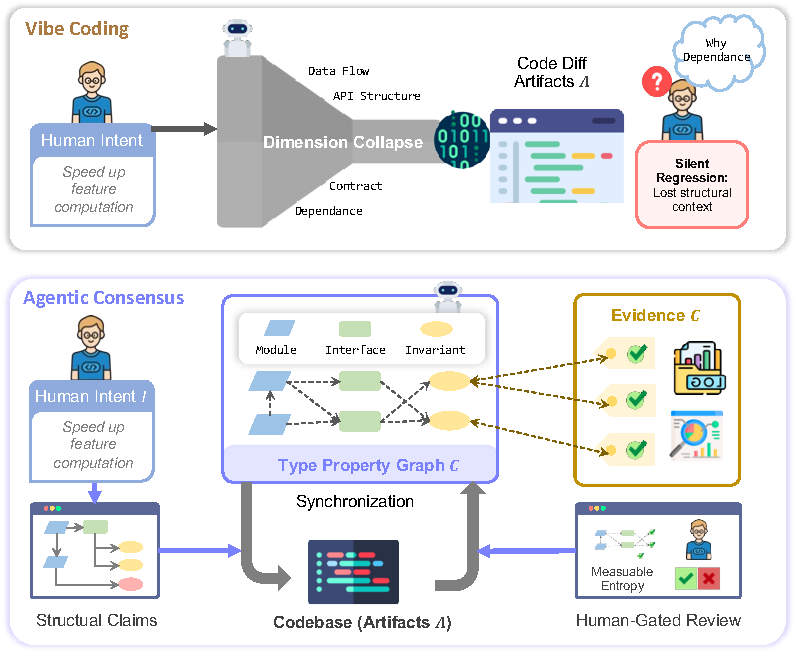
\includegraphics[width=\columnwidth]{figures/consenus-comparison.pdf}
  \caption{Vibe coding (top) treats natural-language prompts as the primary interface and produces code directly, with no persistent structure linking intent to artifacts. Agentic Consensus (bottom) introduces an explicit consensus layer $C$ that mediates between human intent and executable artifacts, maintaining structural traceability and evidence-linked validation throughout the workflow.}
  \label{fig:comparison}
\end{figure}

We propose \textbf{Agentic Consensus} as shown in Figure~\ref{fig:comparison}: a paradigm that replaces ``hoping the AI understood the vibe'' with explicit, operable agreement between humans and machines.
The paradigm shift is to make the consensus layer $C$ the primary artifact of engineering, from which executable artifacts are derived. $C$ is a dynamic, semi-structured operable world model represented as a typed property graph.
Executable artifacts (code, configuration, dataflows) are derived from this shared structure and kept in bi-directional correspondence with it. Linked evidence (tests, checks, traces, provenance) makes every structural claim auditable \cite{chan2024visibility,rasmussen2025zep}.
Programming is thereby reframed as negotiating and validating structural knowledge: entities, dependencies, invariants, and evidence.
The end-state is not ``code that compiles'' but ``structure we agree on.''

\paragraph{Contributions.}
Agentic Consensus is, at its core, a knowledge discovery problem: rehydrating $C$ from artifacts is structure mining; navigating $C$ under uncertainty is graph query answering; evolving $C$ from interaction traces is temporal pattern discovery.
This paper makes four arguments at the intersection of knowledge representation and the emerging challenge of human-AI control:
\begin{itemize}[leftmargin=*, itemsep=2pt]
  \item We argue that the consensus layer $C$ should be the primary artifact of AI-assisted engineering, a structured latent variable mediating between human intent and executable artifacts.
  \item We argue that bidirectional synchronization operators $\Phi$ (realize) and $\Psi$ (rehydrate) are first-class properties that must be continuously executed to maintain consistency between $C$ and $A$
  \item We argue that evaluation must shift from generation quality to alignment and control: alignment fidelity, consensus entropy, intervention distance, and cognitive load reduction.
  \item We propose benchmark task families explicitly designed to measure whether consensus-based workflows reduce human intervention compared to chat-driven baselines.
\end{itemize}


\section{Related Work}
Agentic Consensus draws on multiple threads that each address a facet of the representation gap.

\textbf{Structural Representations for Code.}
Literate programming reframes programs as explanations with executable substructure \cite{knuth1984}. Executable Knowledge Graphs (xKG) extend this by pairing conceptual nodes with runnable code snippets, enabling verifiable replication \cite{luo2025xkg}.
Software modeling (UML-style diagrams) recognizes that engineers reason over graphs, but views are typically illustrative, not synchronized.
Documentation practices (from architecture decision records to doc-as-code pipelines) attempt to preserve design rationale alongside artifacts, but remain passive secondary records: they decay as code evolves, are not bidirectionally linked to implementation, and cannot be operated on by agents.
Our proposal requires bidirectional consistency between views and artifacts \cite{czarnecki2009bidirectional}. Recent structural-LLM work (code property graphs bridged to frozen LLMs \cite{yamaguchi2014cpg,chen2025cgbridge} and typed code DAGs \cite{chivukula2025agint}) demonstrates that explicit graph representations improve semantic fidelity at the code level. Agentic Consensus lifts this idea to the full project state $(I,C,A,E)$, adding evidence linkage and uncertainty tracking.

\textbf{Trust in Agentic Software Engineering.}
Formal methods show that explicit state models support scalable assurance \cite{clarke1999}; the SAFE-AI framework layers safety, auditability, and explainability practices for LLM-assisted SE \cite{navneet2025safeai}.
AIDev's large-scale dataset of 456{,}000 agent-produced PRs reveals that agent changes are accepted significantly less often than human ones \cite{li2025aidev}, and agentic refactoring concentrates on low-level edits rather than structural design changes \cite{horikawa2025refactoring}; this is the trust--utility gap a governable consensus layer targets \cite{lee2004trust}.
Coordination failures between agents mirror classic software risk \cite{brooks1975}. Recent multi-agent SE frameworks establish specialized roles and iterative refinement \cite{hong2024metagpt,qian2024chatdev,bandara2025agentsway,guo2025agentsesurvey}, but maintain consistency via message protocols rather than shared structure.

\textbf{Human--AI Coding Benchmarks.}
SWE-bench \cite{jimenez2024swebench} focuses on single-PR fixes and underestimates realistic complexity. FeatureBench exposes a major gap (11\% on multi-commit features vs.\ 74\% on SWE-bench \cite{zhou2026featurebench}), motivating evaluation beyond pass@$k$.
HAI-Eval introduces ``Collaboration-Necessary'' tasks and measures human--AI synergy across intervention levels \cite{luo2025haieval}, directly compatible with our intervention-distance and cognitive-load metrics.


\section{Agentic Consensus: The Case for a Primary Engineering Artifact}

Human control over AI-generated systems requires a primary artifact that encodes structural commitments. Code encodes only execution; the consensus layer $C$ fills this gap.

\subsection{Structural Artifact Foundations}

\subsubsection{$C$ as the Coordinating Artifact}
We model a project state as a tuple $(I, C, A, E)$:
\begin{itemize}[leftmargin=*, itemsep=2pt]
  \item $I$: user intent, potentially partial, implicit, and time-varying,
  \item $C$: a structured consensus layer (schema, graph, views),
  \item $A$: realized artifacts that execute in the world (code, configs, dataflows), and
  \item $E$: evidence linked to claims in $C$ (tests, traces, provenance).
\end{itemize}
Although the four components are defined together, they are not peers: $C$ is the management layer through which the other three become coherent.
$I$ enters the system through propose/clarify operations that encode intent into structural claims within $C$.
$A$ is derived from $C$ via the realization operator $\Phi$; without $C$, code exists but lacks an auditable rationale.
$E$ attaches to claims in $C$ as validation signals; without $C$, test results are disconnected observations rather than evidence for or against specific commitments.
In short, without $C$ the remaining components are individually meaningful but collectively uncoordinated and unauditable.

\subsubsection{$C$ as an Auditable Graph}
The consensus layer is not a single diagram; it is a typed, queryable schema with multiple synchronized projections.
In practice, $C$ is a labeled property graph whose nodes represent modules, interfaces, data entities, and invariants; edges represent dependencies, contracts, and temporal relations.

%% \begin{figure*}[t]
%%   \centering
%%   \begin{tikzpicture}[
%%     node distance=6mm and 18mm,
%%     nd-human/.style={
%%       draw=black!70, fill=black!6, rounded corners=4pt,
%%       inner sep=6pt, align=center, font=\small,
%%       minimum width=32mm, minimum height=10mm
%%     },
%%     nd-center/.style={
%%       draw=black!85, fill=black!14, rounded corners=4pt,
%%       inner sep=7pt, align=center, font=\small\bfseries,
%%       minimum width=46mm, minimum height=14mm, thick
%%     },
%%     nd-artifact/.style={
%%       draw=black!70, fill=black!6, rounded corners=4pt,
%%       inner sep=6pt, align=center, font=\small,
%%       minimum width=32mm, minimum height=10mm
%%     },
%%     nd-evidence/.style={
%%       draw=black!55, fill=black!3, rounded corners=3pt,
%%       inner sep=5pt, align=center, font=\footnotesize,
%%       minimum width=32mm, minimum height=9mm, dashed
%%     },
%%     nd-views/.style={
%%       draw=black!55, fill=black!3, rounded corners=3pt,
%%       inner sep=5pt, align=center, font=\footnotesize,
%%       minimum width=46mm, minimum height=9mm, dashed
%%     },
%%     ar-main/.style={-{Latex[length=2.5mm, width=2mm]}, thick},
%%     ar-back/.style={-{Latex[length=2.5mm, width=2mm]}, thick, dashed},
%%     ar-evid/.style={-{Latex[length=2mm, width=1.5mm]}, thin, draw=black!50},
%%     nd-lbl/.style={font=\footnotesize, inner sep=2pt, fill=white}
%%   ]
%%
%%   %% ── Row 1: Intent | Consensus Layer | Artifacts ──
%%   \node[nd-human]    (intent)
%%         {Intent $I$\\\footnotesize{(natural language, pointing)}};
%%   \node[nd-center, right=of intent] (C)
%%         {Consensus Layer $C$\\\normalfont\footnotesize{typed property graph,}\\
%%          \footnotesize{schema + synchronized views}};
%%   \node[nd-artifact, right=of C] (artifacts)
%%         {Artifacts $A$\\\footnotesize{code, configs, dataflows}};
%%
%%   %% ── Row 2: Views under C | Evidence under A ──
%%   \node[nd-views, below=of C] (views)
%%         {Multi-modal projections\\\footnotesize{topology, lineage, experiments,}\\
%%          \footnotesize{contracts, causal paths}};
%%   \node[nd-evidence, below=of artifacts] (evidence)
%%         {Evidence $E$\\\footnotesize{tests, checks, traces, provenance}};
%%
%%   %% ── Main horizontal arrows ──
%%   \draw[ar-main] (intent) -- node[nd-lbl, above]{propose / clarify} (C);
%%   \draw[ar-main] (C)      -- node[nd-lbl, above]{$\Phi$\;{\normalfont\footnotesize realize}} (artifacts);
%%   \draw[ar-back] (artifacts) to [bend left=28]
%%                  node[nd-lbl, below]{$\Psi$\;{\normalfont\footnotesize rehydrate}} (C);
%%
%%   %% ── Vertical arrows ──
%%   \draw[ar-evid] (C)         -- (views);
%%   \draw[ar-evid] (artifacts) -- (evidence);
%%   \draw[ar-evid] (evidence.west) to [bend right=20]
%%                  node[nd-lbl, left]{\footnotesize link} (C.south east);
%%
%%   %% ── Human review feedback loop ──
%%   \draw[ar-back] (C.north west) to [bend left=35]
%%                  node[nd-lbl, above]{\footnotesize review / commit / rollback} (intent.north east);
%%
%%   %% ── Dashed boundary around C + views (the "Consensus Zone") ──
%%   \node[draw=black!55, dashed, rounded corners=6pt,
%%         fit=(C)(views), inner sep=8pt,
%%         label={[font=\footnotesize, text=black!60]above right:Consensus Zone}] {};
%%
%%   %% ── Distinguishing annotation ──
%%   \node[font=\footnotesize, text=black!60, align=left,
%%         below=5mm of views, xshift=16mm]
%%         {\textit{Differs from UML / notebooks:}\quad
%%          (i)~round-trip $\Phi$/$\Psi$ operators\quad
%%          (ii)~evidence-linked claims\quad
%%          (iii)~entropy-driven clarification};
%%
%%   \end{tikzpicture}
%%   \caption{%
%%     Architecture of Agentic Consensus.
%%     The consensus layer $C$ (bold center) is the primary artifact;
%%     executable artifacts $A$ are derived via $\Phi$ (realize) and
%%     kept in round-trip correspondence via $\Psi$ (rehydrate).
%%     Evidence $E$ links directly to structural claims in $C$, making every
%%     commitment auditable.
%%     Humans review and commit at the level of $C$, not raw diffs.%
%%   }
%%   \label{fig:canvas}
%% \end{figure*}

\begin{figure*}[t]
  \centering
  % 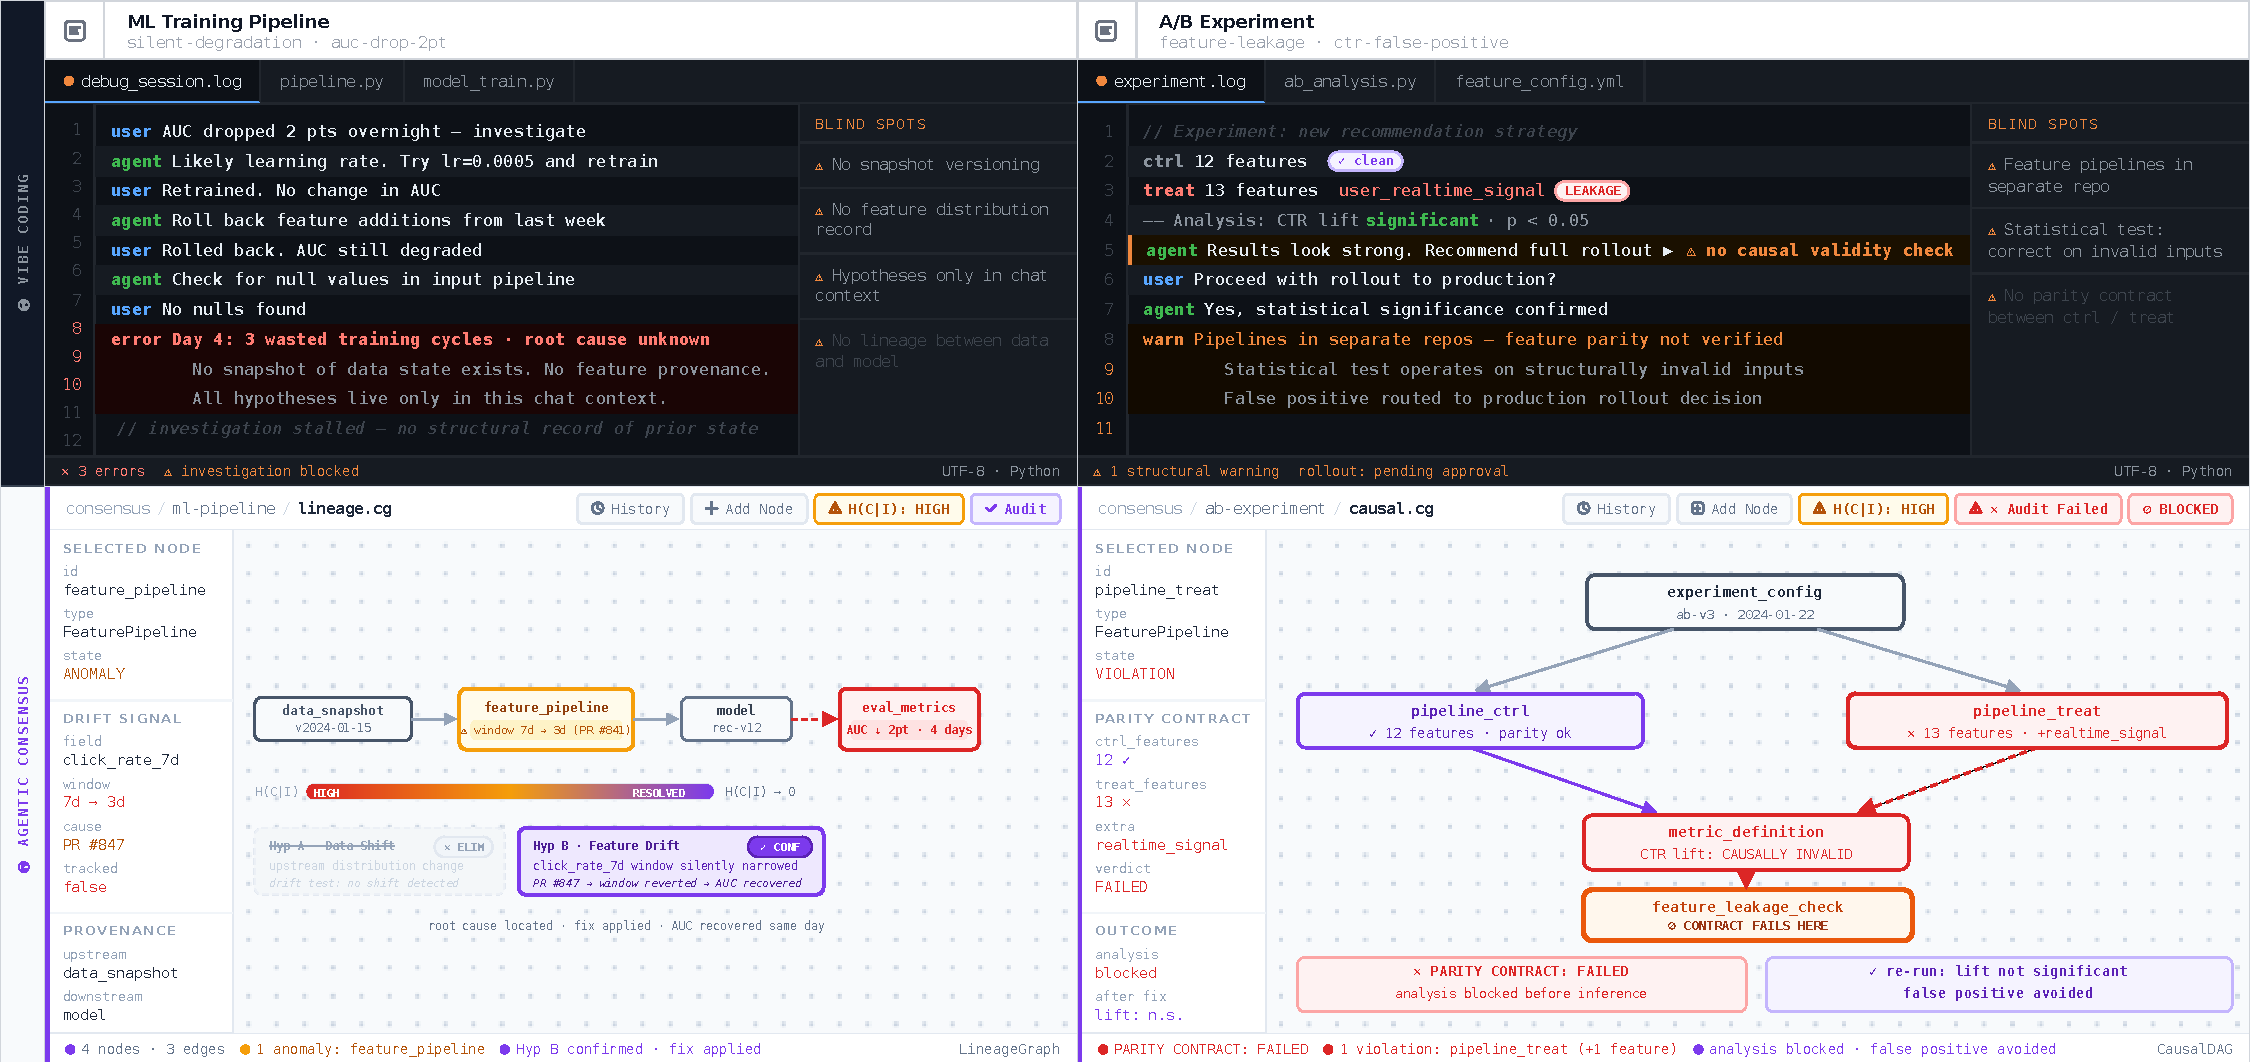
\includegraphics[width=\textwidth]{figures/figure-cases.pdf}
  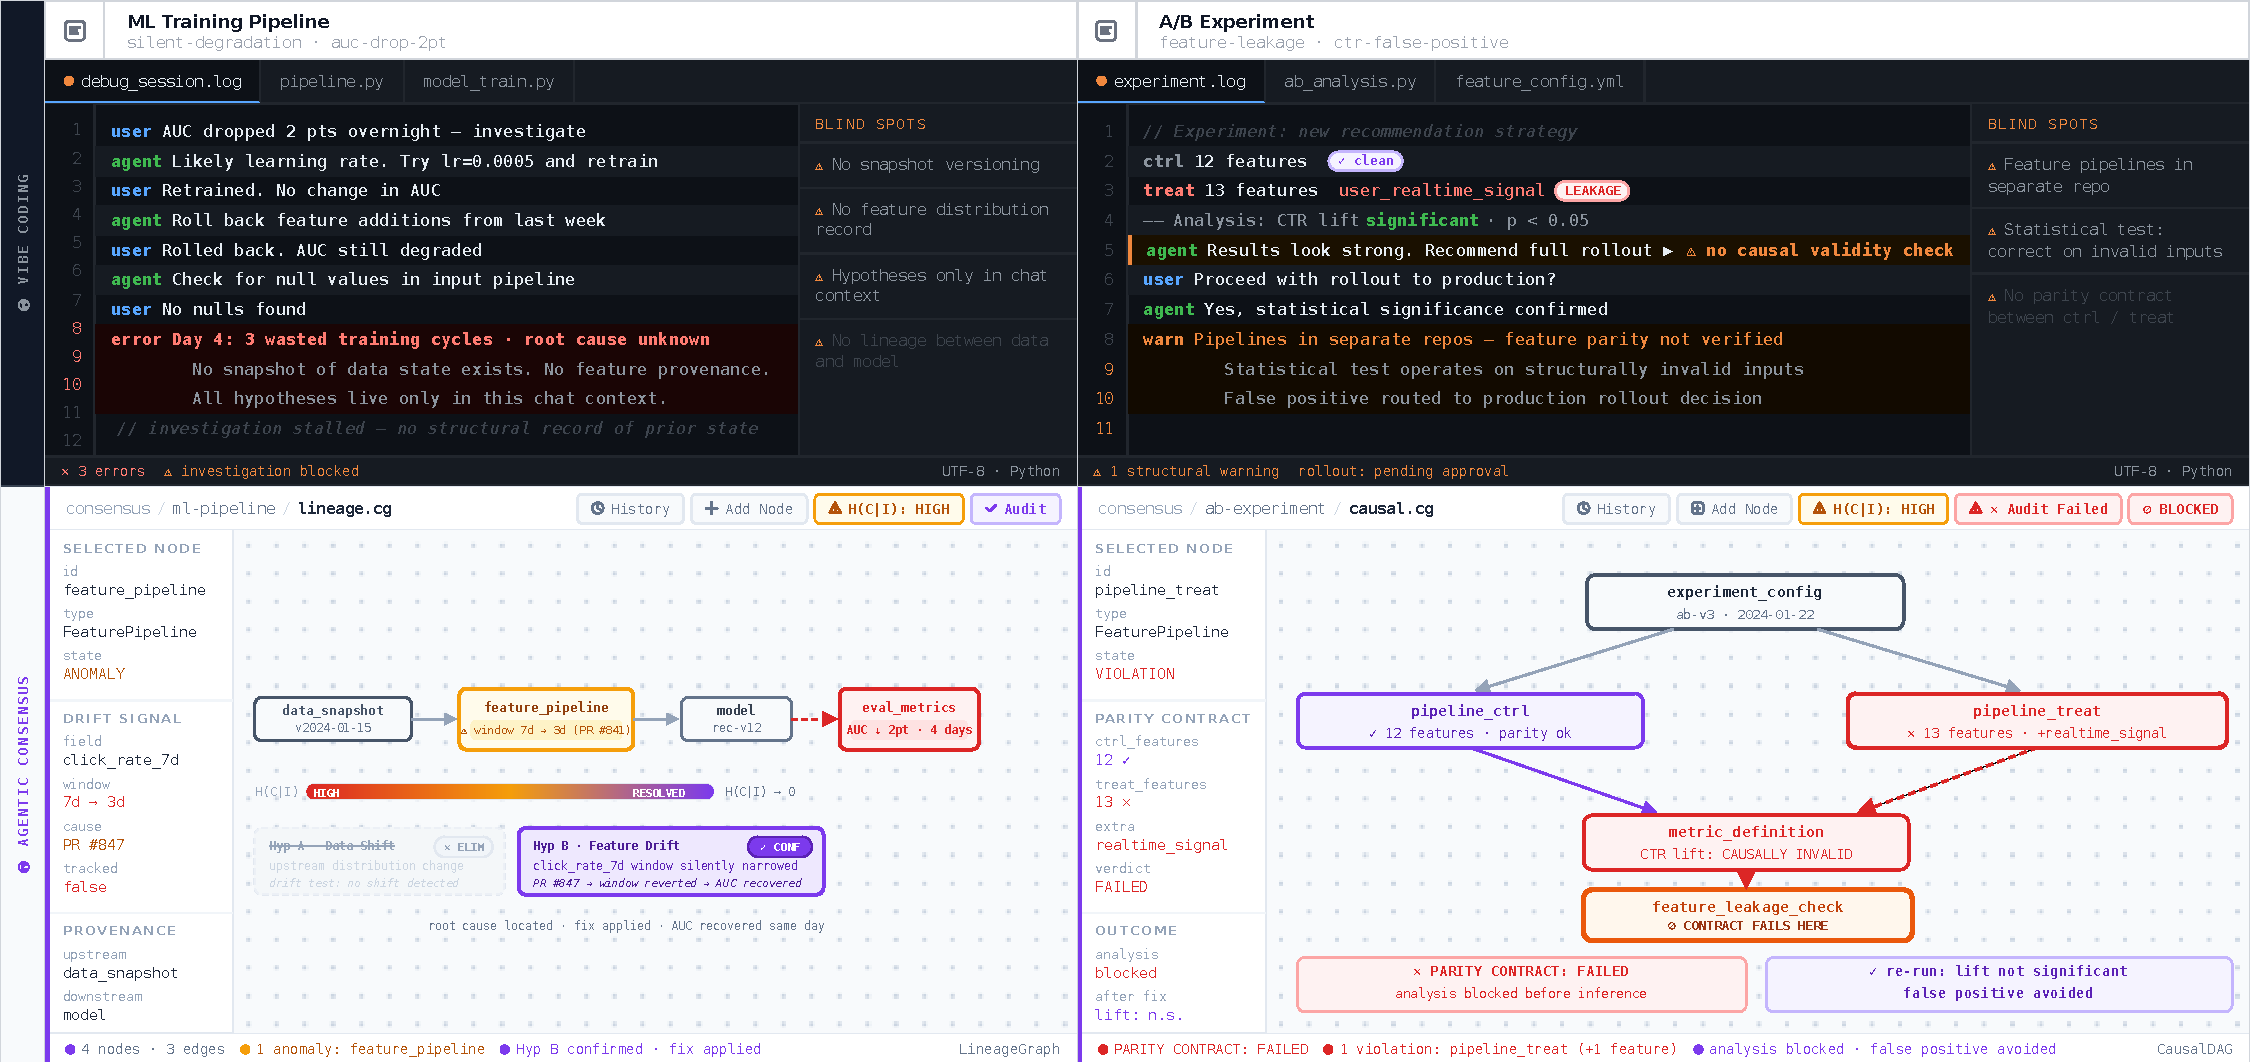
\includegraphics[width=0.90\textwidth]{figures/figure-cases.pdf}
  \caption{Two case studies contrasting vibe coding (left sub-panels) with Agentic Consensus (right sub-panels). \textbf{Case~1} (left): an ML training pipeline's silent AUC degradation---vibe coding produces scattered, context-free debugging sessions, while $C$ maintains pipeline lineage and resolves the root cause (a feature window drift in PR~\#847) within hours. \textbf{Case~2} (right): an A/B experiment with hidden feature leakage---vibe coding approves a statistically significant but causally invalid lift, while $C$'s causal DAG enforces a feature parity contract that blocks rollout before inference begins.}
  \label{fig:democases}
  \vspace{-16pt}
\end{figure*}

Evidence is not a passive record; it is a first-class attribute of the graph, linked directly to claims in $C$.
For example, an edge ``dataset $D$ conforms to schema $S$'' should have pointers to validation jobs and their timestamps.
This auditability requires a precise correspondence between graph elements and artifacts:
\begin{itemize}[leftmargin=*, itemsep=2pt]
  \item \textit{Structural mapping:} nodes map to code units (packages, classes, functions), configuration blocks, or dataset definitions.
  \item \textit{Behavioral mapping:} edges map to explicit call sites, API contracts, data lineage, or testable invariants.
  \item \textit{Round-trip integrity:} changes in $C$ compile down to edits in $A$; changes in $A$ rehydrate back into $C$ via static analysis, runtime traces, and provenance logs.
\end{itemize}

\subsubsection{$C$ as an Operable Sandbox}
$C$ is where agents reason about structure: manipulating dependencies, running analyses, and evaluating counterfactuals without modifying artifacts.

For instance, the system should answer questions of the form:
\begin{quote}
If I delete this node in the consensus graph, which dependencies will break in the downstream code?
\end{quote}

Operationally, this requires that $C$ encodes enough dependency information (and links to evidence) to support ``what-if'' queries and rollback-safe planning.
If the answer depends on unknown or implicit dependencies, that ambiguity should appear as increased consensus entropy rather than as a silent guess.
$C$ also supports context-aware view synthesis: task-relevant subgraphs are projected on demand rather than exposing full topology, keeping $C$ cognitively tractable at scale.

\subsection{Round-Trip Synchronization Requirements}
Structural commitments in $C$ are useful only if they stay in correspondence with artifacts. This requires synchronization to be a first-class system property, not an optional documentation step.

\subsubsection{Synchronization as a First-Class Property}
A session alternates between consensus moves (proposing or modifying $C$) and realization moves (editing $A$ and rehydrating back into $C$). Synchronization operators couple these moves, preserving round-trip integrity and updating evidence links.
We posit two principal operators:
\begin{itemize}[leftmargin=*, itemsep=2pt]
  \item $\Phi: (C, A) \rightarrow A'$ \quad (\emph{realize}): given the current artifact baseline $A$, compile a proposed consensus change into incremental diffs.
  \item $\Psi: (A, C) \rightarrow C'$ \quad (\emph{rehydrate}): infer/update consensus structure from observed artifact diffs.
\end{itemize}
In practice, $\Psi$ is implemented via static analysis (e.g., AST) \cite{yamaguchi2014cpg}, dynamic invariant detection \cite{ernst2007daikon}, data lineage/provenance, and test results. These operators must run continuously, not as on-demand documentation scripts.

\subsubsection{Round-Trip Consistency as a Monitored Approximation}
Ideally, $\Psi(\Phi(C, A)) \approx C$: realizing a consensus change and rehydrating the result should recover the original structure.
In practice, strict equality is unattainable because $\Phi$ may discard structural information that has no artifact-level counterpart, and $\Psi$ is underdetermined.
We therefore treat round-trip consistency as a \emph{soft invariant}: the system continuously measures structural drift $d(C, \Psi(\Phi(C,A)))$ and flags divergence above a threshold, rather than demanding exact isomorphism.
This relaxation is essential for incremental adoption: partial consensus layers provide value before full round-trip fidelity.

When ambiguous, $\Psi$ produces ranked candidate deltas; the system runs cheap discriminating checks (type/schema checks, unit tests, static analyses) and escalates to human input when uncertainty remains high, increasing $\mathcal{H}(C\mid I)$ rather than making a silent guess. Tuning this threshold remains open, as it must balance the cost of interrupting the developer against the risk of silently misattributing intent. 

\subsubsection{Human-Gated Review as a Control Surface}
Every proposed $\Delta C$ arrives with predicted $\Delta A$ and attached evidence; the human decision is gated on structure, not code.
The critical operation is commit/rollback: $\Delta A$ is available for audit and trust calibration but is not the primary review surface.

\subsection{Autonomous Agentic Orchestration}
No single model can maintain $C$ reliably across the full scope of a project. Specialization is necessary: different agents must own different responsibilities over $C$, and their coordination must itself be mediated through $C$ rather than through opaque message exchange.

\subsubsection{Coordinated Multi-Agent Pipelines}
We propose a coordinated pipeline of specialized agents that operate over $C$ and $A$.
This decomposition is informed by emerging multi-agent software-development systems, while shifting the locus of control to a governable consensus artifact $C$ \cite{hong2024metagpt,qian2024chatdev,li2025aidev,wang2025genmentor}.
A representative decomposition uses four roles: an Architect translates intent into structure; a Builder implements artifacts; an Auditor generates evidence and detects conflicts; a Navigator projects the slice of $C$ relevant to the current task. Each agent operates over $C$ as the shared coordination surface rather than through message exchange alone.
Commit/Rollback remains a human decision in all cases.

\subsubsection{Agent--Agent Consensus}
Agents negotiate using richer internal representations, but every outcome is projected back into $C$ before commitment. Conflicts surface as competing $\Delta C$ alternatives with natural-language rationale, highlighted affected paths, and predicted test outcomes; humans commit or reject.

\subsubsection{Expert-Guided Evolution}
Agents that mine interaction traces to discover structural patterns can progressively reduce human intervention distance. 
If recurring corrections cluster around predictable missing relations, the system learns to make those relations first-class in $C$.
This transforms $C$ from a static record into a living knowledge base that grows more accurate as the project evolves and human feedback accumulates.


\section{Case Studies}
We present two illustrative scenarios grounded in patterns commonly observed in data mining practice, shown in Figure~\ref{fig:democases}.

\subsection{ML Training Pipeline: Silent Degradation}

\textit{Setup.} A recommendation model's weekly AUC drops 2 points.
Three days of chat-driven debugging (learning rate tuning, feature rollback, null checks) produce no recovery; each session restarts without knowing what prior attempts ruled out.

\textit{What vibe coding misses.} Root cause is invisible: \texttt{click\_rate\_7d}'s computation window silently changed from 7d to 3d as a side-effect of an unrelated PR, and no links the feature to its consuming model.

\textit{How $C$ responds.} $C$ maintains pipeline lineage (\texttt{data\_snapshot} $\to$ \texttt{feature\_pipeline} $\to$ \texttt{model} $\to$ \texttt{eval\_metrics}) and constructs two competing hypotheses, each with required discriminating evidence: (A)~data shift; (B)~feature drift.
Because $\mathcal{H}(C \mid I)$ is high, the system requests two targeted checks rather than guessing.
Within hours: (A) is eliminated; (B) is confirmed by drift test and traced via $\Psi$ to PR~\#847.
Fix: revert window to 7d. AUC recovers the same day.

\textit{Outcome.} Vibe coding: 4 days, 3 wasted training cycles, root cause unknown.
Agentic Consensus: root cause located and fixed within hours; the fix is recorded in $C$ as evidence for future changes.

\subsection{A/B Experiment: Feature Leakage}

\textit{Setup.} A new recommendation strategy yields a statistically significant CTR lift.
The agent recommends full rollout.

\textit{What vibe coding misses.} Treatment has 13 features; control has 12. The extra feature, \texttt{user\_realtime\_signal}, exists only in treatment: the lift measures feature advantage, not strategy advantage. The agent cannot see the feature pipelines, which live in a separate repo.

\textit{How $C$ responds.} $C$ maintains an experiment causal DAG: the \texttt{experiment\_config} feeds both the control and treatment feature pipelines, which in turn feed \texttt{metric\_definition}.
Before any number is produced, the auditor checks the feature parity contract; it fails.
The analysis is blocked. After removing \texttt{user\_realtime\_signal} and re-running, lift is not significant. The strategy does not work.

\textit{Outcome.} Without $C$, a false positive triggers full rollout and takes 2--3 weeks in production to expose; with $C$, the structural violation is caught before inference begins.
The original result was statistically correct but causally invalid; a more capable model would have produced the same wrong answer.

\paragraph{What these cases demonstrate.}
The first case shows $C$ as a \emph{diagnosis surface}: hypotheses are explicit, entropy is measurable, and evidence collapses uncertainty.
The second shows $C$ as a \emph{validity gate}: structural contracts block causally invalid conclusions before they are produced.
In both cases the failure is not generative; it is structural. As AI throughput scales, opacity accumulates faster than humans can inspect it; without a governable consensus layer, scaled AI-assisted engineering degrades into scaled opacity.


\section{Evaluation Framework}
Evaluating Agentic Consensus requires moving beyond code correctness (pass@$k$) toward four complementary metrics that measure structure, uncertainty, and human control.
\textit{(a) Alignment fidelity} $\mathcal{F}(I,C,A)$ increases when $C$ makes intent explicit at the right abstraction level and is predictive (reviewers can anticipate downstream consequences); it can be estimated via human annotations, counterfactual questions, and post-hoc blame assignment.
\textit{(b) Consensus entropy} $\mathcal{H}(C\mid I)$ quantifies structural ambiguity given current intent; we use conditional-entropy notation as conceptual shorthand rather than a literal Shannon quantity. High $\mathcal{H}$ is not failure; it is a signal to switch from execution to clarification.
\textit{(c) Intervention distance} counts the number and complexity of human corrections needed to reach a correct consensus state.
\textit{(d) Cognitive load} measures whether humans understand systems faster by interacting with $C$ than by reading raw artifacts \cite{sweller1988cognitive,klein2005common,siemon2022taxonomy,lee2004trust}.

\paragraph{\textbf{Benchmark design.}}
We propose task families explicitly designed for consensus-based workflows: refactor-with-invariants (restructure while preserving contracts), failure localization (update $C$ with the true causal path), experiment design (represent and validate ablation plans in $C$), and governance tasks (implement policy changes where success requires correct structure, not just passing tests).
FeatureBench's multi-commit tasks \cite{zhou2026featurebench} and HAI-Eval's collaboration-necessary protocol \cite{luo2025haieval} provide compatible task distributions and human-collaboration protocols for external validation.


\section{Discussion}

\subsection{Alternative Views}
We address three substantive objections to Agentic Consensus.

\paragraph{``Better models will solve this without a consensus layer.''}
One might argue that sufficiently capable agents will internalize system structure implicitly, making explicit representation unnecessary.
Structurally, the problem is not model capability but human legibility. Even a perfect model that silently maintains a correct internal world model cannot provide the transparency, auditability, and governance that human-AI collaboration requires.
The consensus layer is not a crutch for weak models. It is the interface through which humans exercise meaningful control regardless of model quality.
As models improve, the consensus layer becomes easier to maintain, not unnecessary.
More capable models can produce statistically valid outputs on structurally invalid inputs, and the failure mode becomes harder to detect as scale grows.

\paragraph{``$\Psi$ will hallucinate, making $C$ unreliable.''}
This is a real risk, and we address it by design.
$\Psi$ does not produce a single deterministic rehydrated graph. It produces candidate deltas $\{\Delta C_1, \Delta C_2, \ldots\}$ with uncertainty scores.
Ambiguous rehydration increases $\mathcal{H}(C \mid I)$ and triggers clarification rather than silent reinterpretation.
Round-trip consistency is treated as a soft invariant. The system monitors structural drift $d(C, \Psi(\Phi(C, A)))$ and flags divergence above a threshold rather than demanding exact isomorphism.
Hallucinated structure becomes visible as unsupported claims in $C$ that evidence links fail to corroborate.
The historical failure of UML synchronization tools is instructive but not analogous. Those tools required human maintenance of a secondary artifact. $\Phi$ and $\Psi$ are agent-executed operators running continuously, removing the cost that caused UML to decay.
An escape hatch for low-overhead changes remains a necessary design requirement.

\paragraph{``Graph-based representations are brittle for dynamic, exploratory work.''}
Early-stage exploratory coding is inherently unstructured, and imposing graph schemas too early is a real constraint on creativity. We do not propose that Agentic Consensus applies to all workflows uniformly.
The consensus layer should be incrementally adoptable. Systems begin with partial, low-confidence structure and tighten it as projects stabilize.
High consensus entropy is a signal to not impose structure yet, not a failure.
On cognitive load: $C$ is never exposed as a raw graph. The navigator projects task-relevant subgraphs on demand, so what humans review is a structured summary of the relevant slice, not the full topology.

\subsection{Limitations}
Agentic Consensus raises practical concerns in two areas: system reliability and real-world deployment.

\paragraph{Runtime Risks.}
Agentic Consensus requires careful governance: access control over $C$, redaction for sharing, and escape hatches for low-friction work when structure is unnecessary.
Agents may hallucinate structure; these failures should be visible as high-entropy regions and blocked by required evidence. Evidence itself is not infallible (tests can be flaky, traces noisy, static analyses prone to false positives), so each evidence link in $E$ should carry a confidence weight and contradictory evidence should surface as an explicit inconsistency in $C$, not be silently resolved.

\paragraph{Progressive Adoption.}
For large legacy systems, full rehydration is intractable; $\Psi$ must instead bootstrap incrementally, covering critical modules first and expanding as engineers interact with the system, with uncovered regions marked as high-entropy zones.
For large codebases, $C$ need not be monolithic: sub-graph partitioning along package or service boundaries lets each agent operate on a local view, with the same ownership boundaries that govern human collaboration governing agent coordination.

\subsection{Broader Implications}
Although motivated by coding, Agentic Consensus generalizes to any knowledge discovery system where agents autonomously discover, visualize, and synchronize latent structure in complex datasets or socio-technical systems for human oversight and~intervention.


\section{Conclusion}
Agentic Consensus reframes system building as a collaborative discovery process on shared, verifiable structure.
It replaces ``hoping the AI understood the vibe'' with explicit, operable agreement between humans and machines.
The deeper question it raises is not technical but epistemological: as AI systems become capable of generating artifacts faster than humans can inspect them, what is the right unit of human oversight?
We argue it is not the line of code, not the diff, and not the chat message. It is the structural claim, made explicit, linked to evidence, and kept in agreement with the world.
Building the infrastructure for that agreement is a foundational open problem for knowledge representation and human-AI collaboration systems.



\bibliographystyle{ACM-Reference-Format}
\bibliography{main}

\appendix



\end{document}
\endinput
%%
%% End of file `sample-sigconf.tex'.
